% Created 2021-10-28 Thu 09:27
% Intended LaTeX compiler: pdflatex
\documentclass[11pt]{article}
\usepackage[utf8]{inputenc}
\usepackage[T1]{fontenc}
\usepackage{graphicx}
\usepackage{grffile}
\usepackage{longtable}
\usepackage{wrapfig}
\usepackage{rotating}
\usepackage[normalem]{ulem}
\usepackage{amsmath}
\usepackage{textcomp}
\usepackage{amssymb}
\usepackage{capt-of}
\usepackage{hyperref}
\author{Daniel Rosel}
\date{\today}
\title{Frame of Life}
\hypersetup{
 pdfauthor={Daniel Rosel},
 pdftitle={Frame of Life},
 pdfkeywords={},
 pdfsubject={},
 pdfcreator={Emacs 27.1 (Org mode 9.5)}, 
 pdflang={English}}
\begin{document}

\maketitle
\tableofcontents


\section{Introduction}
\label{sec:org1979d4b}
Life perceived simply by ones eyes, can be very chaotic, but when carefully analyzed, there are many patterns which depend on each other. To be able to predict behavior and stack patterns, a ground level of behavioral prediction must be established. Our core day-to-day behavior is highly periodic and can be modeled using simple trigonometric functions.
\section{Mechanics}
\label{sec:org5bc44ce}
Life can be represented as a single line \(y = 2\) and events in life as intersections with that line. Each day, can be mapped out by a function such as:
\begin{equation}
    d = \cos{(\Xi x + \pi) + 1}, (10^{-5} \leq \Xi \leq 10^{5})
\end{equation}
In this case \(\Xi\) is making the system more or less precise. The noon of each day is where \(d \cap y\) and each day ends at \(\Xi2\pi(c)\).
\subsection{Periodic Events in Life}
\label{sec:org2e55719}
Most events in life work on a periodic basis, this can be represented by:
\begin{equation}
s = 1 + \cos{(\frac{1}{n}x + (\sigma)\pi)}
\end{equation}
The above equation can model nearly every even in life.
\begin{itemize}
\item \(n\) is the frequency (in days) of the event.
\item \(\sigma\) is the shift which changes the occurrence of the event in the day \(n\).
\end{itemize}
\subsubsection{Determining temporal proximity relative to certain event}
\label{sec:orgcce3672}
For the implementation of this system in algorithms and neural networks, knowing the proximity of events relative to a certain day (\(n\)), a simple optimization algorithm must be used. For zero-range events, the target is finding an x for which \(\dot{f}(x)\) is 0 and \(f(x) = 2\).

\subsection{Computing the Parameters}
\label{sec:orgbe29fa8}
\subsubsection{zero-range events}
\label{sec:orgaf096b9}
A 0 range event is an event which simply occurs, but does not last any long period of time. To create a function such that it follows our criteria, we must compute sigma.
\begin{equation}
    \sigma = -\frac{\frac{1}{n}x}{\pi}
\end{equation}
In the above equation, it's variables represent the following:
\begin{itemize}
\item \(n\) is the frequency of occurrence (in days)
\item \(x\) is as follows:
\begin{equation}
  x = \frac{h}{24} * 2\pi
\end{equation}
where \(h\) is the hour at which the event occurs.
\end{itemize}
\begin{enumerate}
\item \textbf{Example}
\label{sec:org12f3c5b}
Alice wakes up at 0600 every day. The function for this behavior would look as the following:
\begin{equation}
b = \cos{( x + (\frac{-(\frac{6}{24}*2\pi)}{\pi})\pi )} + 1 = \cos{(x-\frac{1}{4}2\pi)}+1
\end{equation}
\item \textbf{Visualization}
\label{sec:orge7643a4}
Using a Java algorithm, the following is the output of functions compiled given life parameters.
\begin{center}
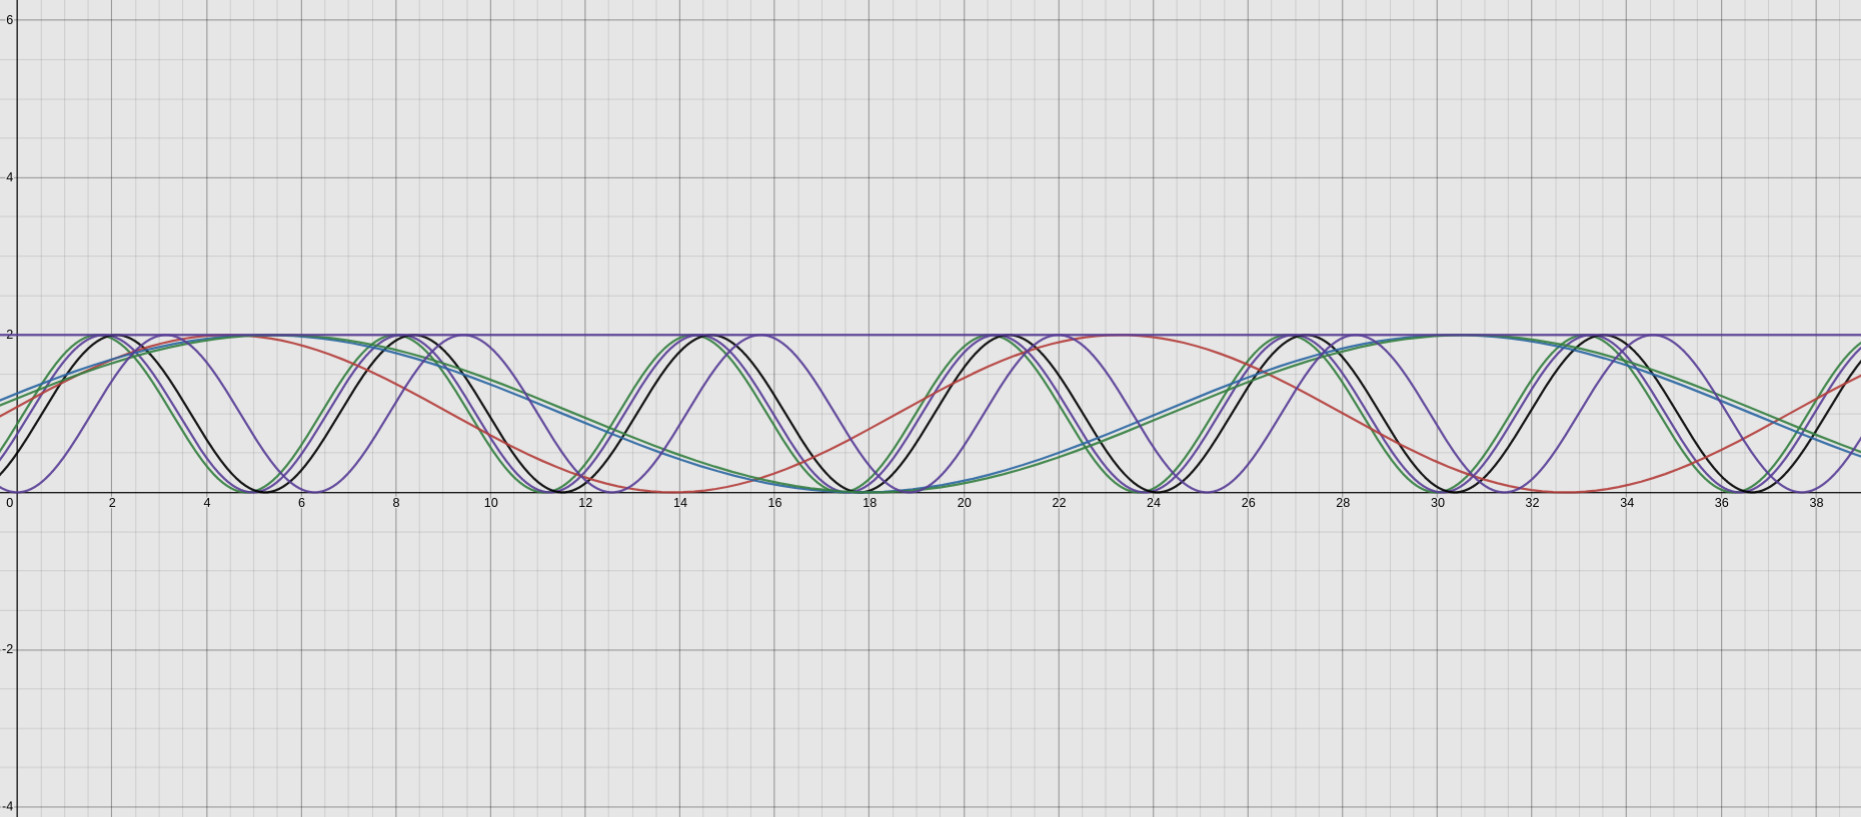
\includegraphics[width=.9\linewidth]{./media/life01.jpg}
\end{center}
\end{enumerate}
\subsubsection{lasting events}
\label{sec:orgfffd6fb}
Events that have a start and an end, can be represented by a set of 2 zero-range events, one as a marker for the start and the other marking the end. Another potential approach would be to scale the function on the y-axis, creating 2 intercepts with \(y=2\), marking the start and end with just one function.
\section{Abstractions}
\label{sec:orgb4b4a5c}
\subsection{Inconsistent behavior}
\label{sec:orga6ad15e}
Not all events happen with a 100 percent certainty.
\subsection{Weekends}
\label{sec:org5ab999d}
The majority of people, do not work each day of the week, but rather Monday \(\to\) Friday. How can we create a special case for every weekend, so that a predicted event does not stand true? We can formulate another event which can be refereed to as a negation event. This event will have a different y-axis shift, making it's implication clearly different.
\begin{enumerate}
\item \textbf{Example}
\label{sec:org6cfdcc7}
\end{enumerate}
\subsection{Subject Busyness}
\label{sec:org2b46bd2}
To see how busy each day of a subjects life is, one can do the following:
\begin{equation}
    f_c(x) = 1 + \sum_{i=0}^{n}{ \cos(s_i_{\text{frequency}}x - s_i_{\sigma} \pi})
\end{equation}
where \(s\) is the function representing an event in a set of \(n\) events. When graphically compared to the day function (\(y = cos(x - \pi) + 1\)), we get the following:
\begin{center}
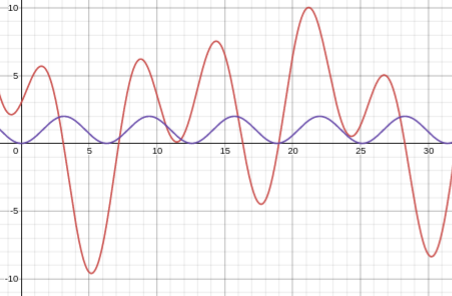
\includegraphics[width=.9\linewidth]{./media/activity_density.png}
\end{center}
With a large enough set of parameters, you will rarely observe a repeating pattern in the composite function;
\end{document}
